\documentclass[10pt]{beamer}
\newcommand \bibPath{../paper_ms_method_HSCY1/}
\newcommand \figPath{../paper_ms_method_HSCY1/}

\usetheme[progressbar=frametitle,numbering=fraction]{metropolis}
\usepackage{appendixnumberbeamer}
\usepackage{appendixnumberbeamer}\usepackage{booktabs}
%\renewcommand{\vec}[1]{\boldsymbol{#1}}

\usepackage[round,sort,comma]{natbib}

\usepackage{graphicx}	% Including figure files
\usepackage{subfigure}
\usepackage{pdflscape}	% Landscape pages
\usepackage{epstopdf}
\usepackage{commath}
\epstopdfsetup{update}
\usepackage{xspace}
\usepackage{soul}

\newcommand{\mathcolorbox}[2]{\colorbox{#1}{$\displaystyle #2$}}
\newcommand{\hlfancy}[2]{\sethlcolor{#1}\hl{#2}}
\newcommand{\themename}{\textbf{\textsc{metropolis}}\xspace}

\usepackage{xcolor}
\definecolor{hellmagenta}{rgb}{1,0.75,0.9}
\definecolor{hellcyan}{rgb}{0.75,1,0.9}
\definecolor{hellgelb}{rgb}{1,1,0.8}
\definecolor{colKeys}{rgb}{0,0,1}
\definecolor{colIdentifier}{rgb}{0,0,0}
\definecolor{colComments}{rgb}{1,0,0}
\definecolor{colString}{rgb}{0,0.5,0}
\definecolor{darkyellow}{rgb}{1,0.9,0}

\title{$3$-D mass map reconstruction with sparsity regularization}
\subtitle{}
 \date{\today}
%\date{2018/06/26}
\author{
Xiangchong Li, Naoki Yoshida, Masamune Oguri,
Shiro Ikeda, Wentao Luo
\\ }

\institute{Department of Physics, University of Tokyo }


\begin{document}

\maketitle



\section{Background}
\begin{frame}{Lensing}
\begin{columns}
\begin{column}{0.5\textwidth}
\begin{alertblock}{From $\delta(z_l)$ to $\gamma(z_s)$}
\begin{equation}\notag
\kappa(\vec{\theta},z_s)= \mathcolorbox{yellow}{\int_0^{z_s} dz_l K(z_l,z_s)}\delta(\vec{\theta},z_l).
\end{equation}

\begin{equation}\notag
K(z_l,z_s) =
\begin{cases}
\frac{3H_0\Omega_M}{2 c} \frac{\chi_l \chi_{sl} (1+z_l)}{\chi_{s} E\left(z_l\right)} & (z_s>z_l),\\
0&(else).
\end{cases}
\end{equation}

\begin{equation}\notag
\gamma^t(\vec{\theta},z_s) = \mathcolorbox{yellow}{\int d^2 \theta' D(\vec{\theta}-\vec{\theta'})} \kappa(\vec{\theta'},z_s) ,
\end{equation}

\begin{equation}\notag
D(\vec{\theta})=-\frac{1}{\pi}(\theta_1-i\theta_2)^{-2}.
\end{equation}

\end{alertblock}
\end{column}
\begin{column}{0.7\textwidth}
\centering
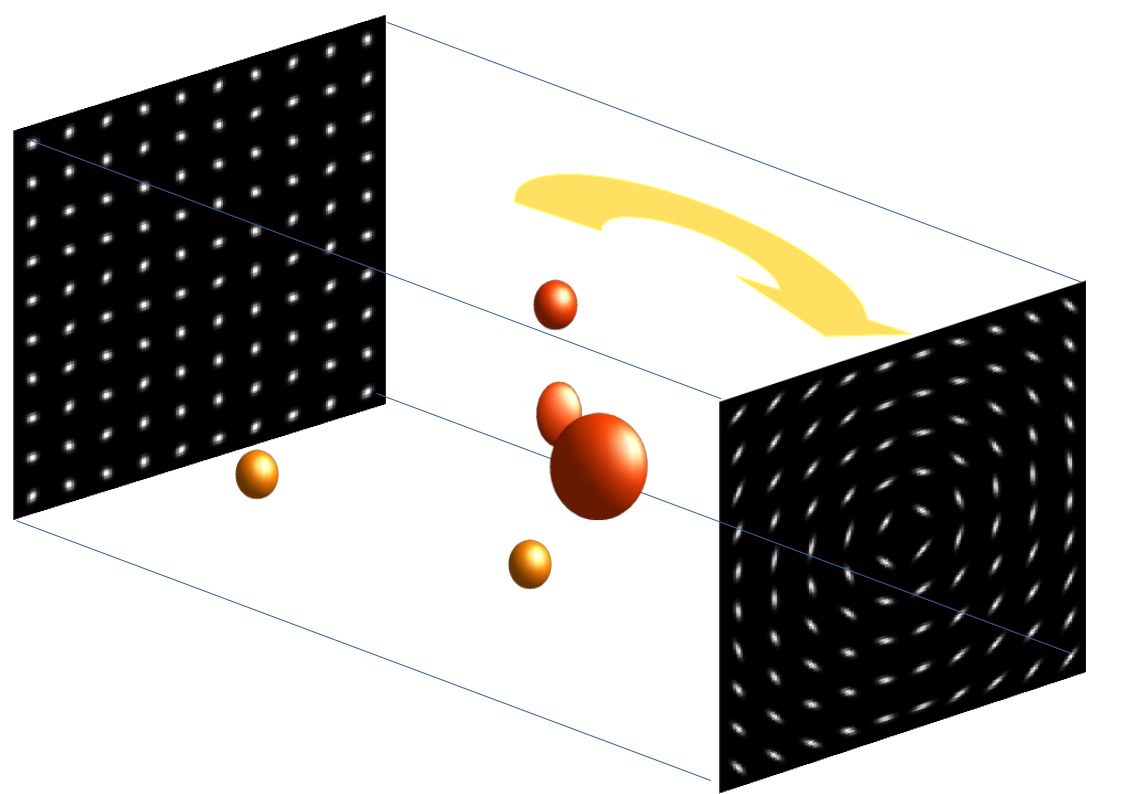
\includegraphics[height=.6\textwidth]{weak_lensing_shear_deom.png}
\end{column}
\end{columns}
\colorbox{cyan}{\small A non-local convolution in both line-of-sight direction and the transverse plane.}
\end{frame}


\begin{frame}{ Model}
\begin{alertblock}{Model space $\phi$}
\begin{equation}\notag
\begin{split}
\delta&=\int d^3 r \phi(\vec{r}) x(\vec{r})\\
\delta&=\mathbf{\Phi} x
\end{split}
\end{equation}
\begin{itemize}
 \item $\phi = \delta_D$
 \begin{itemize}
    \item  2D [Kaiser \& Squires 1995]
 \end{itemize}
 \item $\phi = e^{i\vec{k}\cdot \vec{r}}$
 \begin{itemize}
    \item  Wiener filter (Ridge regularization) [Oguri et. al 2018]
 \end{itemize}
 \item $\phi = \rm{starlets}$
 \begin{itemize}
    \item  lasso sparsity regularization (Glimpse3D) [Leonard et. al 2013]
 \end{itemize}
\end{itemize}

\end{alertblock}
\end{frame}

\begin{frame}{$\chi^2$ fitting}
\begin{alertblock}{Lensing ($\mathbf{DK}$)}
\begin{equation}\notag
\gamma = \mathbf{D} \mathbf{K} \delta
\end{equation}
\end{alertblock}

\begin{alertblock}{Model ($\mathbf{\Phi}$)}
\begin{equation}\notag
\gamma = \mathbf{D} \mathbf{K} \mathbf{\Phi} x + \epsilon
\end{equation}
\end{alertblock}

\begin{alertblock}{Systematics ($\mathbf{S}$)}
\begin{equation}\notag
\gamma = \mathbf{S} \mathbf{D} \mathbf{K} \mathbf{\Phi} x + \epsilon
\end{equation}
\end{alertblock}

\begin{alertblock}{$\chi^2$ fitting}
\begin{equation}\notag
\begin{split}
&\rm{min} \{\norm{\gamma - \mathbf{A}x}^2_2\}\\
& x=(\mathbf{A^TA})^{-1} \mathbf{A^T} \gamma
\end{split}
\end{equation}
\end{alertblock}

\end{frame}


\begin{frame}{Difficulties in the $\chi^2$ fitting}
\begin{alertblock}{ill-posed problem}
\begin{equation}\notag
\begin{split}
&\rm{min} \{\norm{\gamma - \mathbf{A}x}^2_2\}\\
& x=(\mathbf{A^TA})^{-1} \mathbf{A^T} \gamma
\end{split}
\end{equation}

\begin{enumerate}
 \item Shape noise ($\sigma_\gamma \sim 0.3$, $\gamma \sim 0.03$)
 \item Masks (have to do zero padding)
\end{enumerate}

\end{alertblock}

\end{frame}

\begin{frame}{$\chi^2$ fitting with regularization}
\begin{alertblock}{regularizations}
\begin{equation}\notag
\norm{\gamma - \mathbf{A}x}^2_2 + C(x)
\end{equation}

\begin{enumerate}
 \item Ridge regularization (Wiener filter) [Oguri et. al 2018]
 \begin{equation}\notag
  C(x) \sim \norm{x}^2_2
 \end{equation}
 \item Lasso regularization (Glimpse3D) [Leonard et. al 2013]
 \begin{equation}\notag
  C(x) \sim \norm{x}^1_1
 \end{equation}
 \item Total Square Variance (TSV) regularization
 \begin{equation}\notag
  C(x) \sim \sum_i (x_{i+1}-x_{i})^2
 \end{equation}
\end{enumerate}

\end{alertblock}

\end{frame}


\begin{frame}{Bayesian Interpretion of regularization}
\begin{alertblock}{Prior}
\begin{equation}\notag
P(x|\gamma) \propto P(x)P(\gamma|x)
\end{equation}
\end{alertblock}

\begin{columns}
\begin{column}{0.5\textwidth}
\begin{alertblock}{Ridge regularization}
\begin{equation}\notag
P(x) \propto exp(-\norm{x}_2^2)
\end{equation}
\end{alertblock}

\begin{alertblock}{Sparse regularization}
\begin{equation} \notag
P(x) \propto exp(-\norm{x}_1^1)
\end{equation}

\end{alertblock}
\end{column}
\begin{column}{0.6\textwidth}
\centering
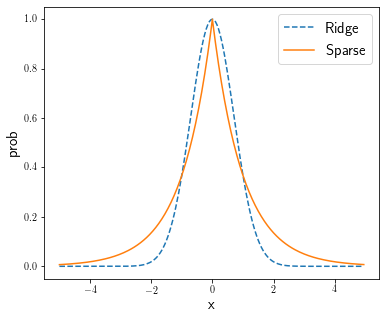
\includegraphics[height=.8\textwidth]{prior_ridge_sparse.png}
\end{column}
\end{columns}
\end{frame}

\begin{frame}{Bayesian Interpretion of regularizations}
\begin{alertblock}{Prior}
\begin{equation}\notag
P(x|\gamma) \propto P(x)P(\gamma|x)
\end{equation}
\end{alertblock}

\begin{columns}
\begin{column}{0.5\textwidth}
\begin{alertblock}{TSV}
\begin{equation}\notag
P(x) \propto exp(-\sum_i (x_i-x_{i+1})^2)
\end{equation}
\end{alertblock}
\end{column}
\begin{column}{0.6\textwidth}
\centering
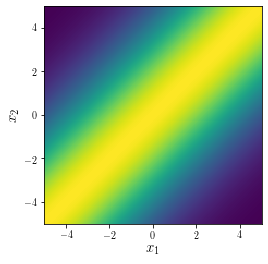
\includegraphics[height=.8\textwidth]{prior_TSV.png}
\end{column}
\end{columns}
\end{frame}

\section{Method}


\begin{frame}{Model Dictionary}

We use surface density profile of [Takada \& Jain (2003)] as the transverse profile of our basis vector.
\begin{equation}\notag
F(r)=
\begin{cases}
-\frac{\sqrt{c^2-r^2}}{(1-r^2)(1+c)} + \frac{\rm{arccosh} \left(\frac{r^2+c}{r(1+c)}\right)}{(1-r^2)^{3/2}}  & (r<1),\\
\frac{\sqrt{c^2-1}}{3(1+c)} (1+\frac{1}{c+1}) & (r=1),\\
-\frac{\sqrt{c^2-r^2}}{(1-r^2)(1+c)} + \frac{\rm{arccos} \left(\frac{r^2+c}{r(1+c)}\right)}{(r^2-1)^{3/2}} & (1<r\leq c),\\
0& (r>c).
\end{cases}
\end{equation}
In the line-of-sight direction, we use Dirac delta function
\begin{equation}\notag
 \phi(\vec{r})=F(|\vec{\theta}|/r_s) \delta_D(z)
\end{equation}
\end{frame}

\begin{frame}{Model Dictionary}
\begin{alertblock}{Smoothed basis vectors}
\begin{figure}
\centering
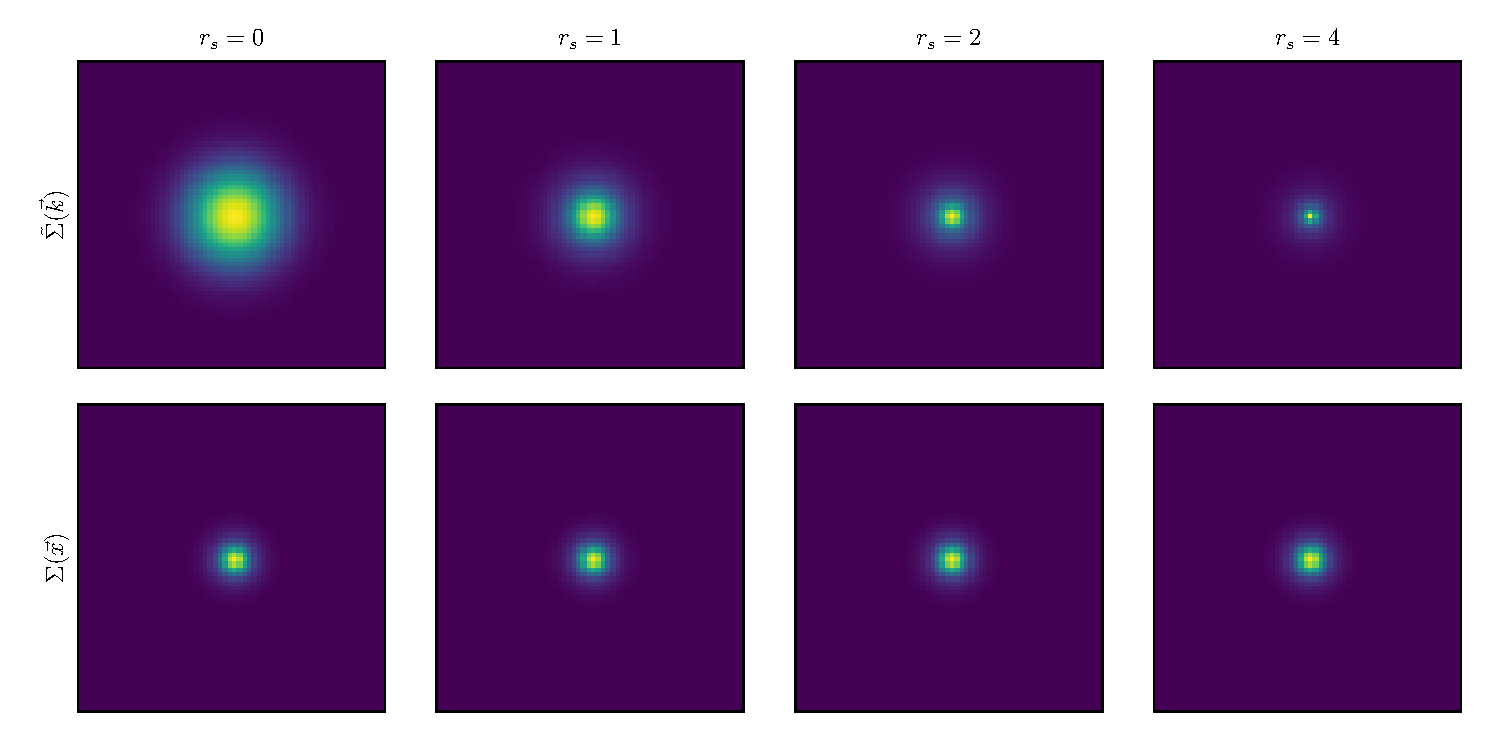
\includegraphics[height=.5\textwidth]{../paper_ms_method_HSCY1/nfwlet-atom-2D.pdf}
\end{figure}

\small pixel size $=1$ arcmin,
\small Gaussian smoothing scale $=1.5$ arcmin,
\small redshift bin $\Delta z=0.05$,
\small $4$ dictionary frames.
The indexing $x[s,i,j,k]$ or $x_\alpha$
\end{alertblock}
\end{frame}


\begin{frame}{Regularized ML Fitting}
\begin{alertblock}{The Loss function}
\begin{equation}\notag
\begin{split}
&L(x) = \mathcolorbox{yellow}{\frac{1}{2} \norm{\gamma-\mathbf{A}x}^2_2} + \\
&\mathcolorbox{yellow}{\frac{1}{2}\tau \sum_{i,j}\left[(x[s,i+1,j,k]-x[s,i,j,k])^2+x[s,i,j+1,k]-x[s,i,j,k])^2\right]}\\
&+\mathcolorbox{cyan}{\lambda \sigma(x) \norm{x}_1}.
\end{split}
\end{equation}
\begin{equation}
\begin{split}
L(x)&=\frac{1}{2}(\gamma_{\alpha}-A^{*}_{\alpha\beta}x_{\beta})(\gamma_{\alpha}-A_{\alpha\mu}x_{\mu})\\
&+\frac{\tau}{2}[(D^{1}_{\alpha\beta} x_{\beta})(D^{1}_{\alpha\mu}x_{\mu})
+ (D^{2}_{\alpha\beta} x_{\beta})(D^{2}_{\alpha\mu}x_{\mu})] \\
&+ \lambda\sigma_\beta \norm{x_\beta}_1,
\end{split}
\end{equation}
where $\mathbf{D^{1,2}}$ refers to finite difference operator. Here we adopt Einstein notation on $\alpha, \beta, \mu, \nu$.
\end{alertblock}
\end{frame}

\begin{frame}{Solving the ML problem}
\begin{alertblock}{The quadratic term}
\begin{equation}\notag
\begin{split}
 G(x)&=\frac{1}{2}(\gamma_{\alpha}-A^{*}_{\alpha\beta}x_{\beta})(\gamma_{\alpha}-A_{\alpha\mu}x_{\mu})\\
&+\frac{\tau}{2}[(D^{1}_{\alpha\beta} x_{\beta})(D^{1}_{\alpha\mu}x_{\mu})
+ (D^{2}_{\alpha\beta} x_{\beta})(D^{2}_{\alpha\mu}x_{\mu})],
\end{split}
\end{equation}
\end{alertblock}
\begin{alertblock}{Coordinate descent Algorithm}
Begin with $x^{(0)}=0$, for one coordinate $t [s,i,j,k]$
\begin{equation}\notag
x^{(n+1)}_{t}=\mathrm{ST}_{\lambda\sigma_{t}} (x^{(n)}_{t} -\frac{\partial_t G(x^{(n)})}{A_{\alpha t}A_{\alpha t}+4\tau}),
\end{equation}
where $\mathrm{ST}$ is the soft thresholding function defined as
\begin{equation}\notag
\mathrm{ST}_{\lambda} (x) = \mathrm{sign} (x) \max (\abs{x}-\lambda,0).
\end{equation}
We set $\lambda=4$, $\tau= \frac{1}{N} \sum_t^N (A_{\alpha t}A_{\alpha t})\times 20$, $\sigma(x)$ the noise expected on projector
$x$.
\end{alertblock}
\end{frame}

\begin{frame}{Solving the ML problem}
\begin{alertblock}{Coordinate descent Algorithm}
\begin{equation}\notag
x^{(n+1)}_{t}=\mathrm{ST}_{\lambda\sigma_{t}} (x^{(n)}_{t} -\frac{\partial_t G(x^{(n)})}{A_{\alpha t}A_{\alpha t}+4\tau}),
\end{equation}
\begin{equation}\notag
\mathrm{ST}_{\lambda} (x) = \mathrm{sign} (x) \max (\abs{x}-\lambda,0).
\end{equation}
\end{alertblock}

\begin{itemize}
\item Begin with $x^{(0)}=0$,
 \item for n=1...$N_{iter}$
    \begin{enumerate}
     \item select one coordinate $t [s,i,j,k]$
     \item $ \bar{x}_t^{(n)}=x^{(n)}_{t} -\frac{\partial_t G(x^{(n)})}{A_{\alpha t}A_{\alpha t}+4\tau}$
     \item \begin{itemize}
            \item if $ \bar{x}_t^{(n)}>\lambda \sigma_t$: $x_t^{(n+1)}=0.$
            \item else: $x_t^{(n+1)}= \bar{x}_t^{(n)}-\lambda\sigma_t$
           \end{itemize}

    \end{enumerate}

\end{itemize}
\end{frame}

\section{Test on HSC-like Simulation}
\begin{frame}{Simulation}
\begin{alertblock}{Binning in line-of-sight direction}

\end{alertblock}
\begin{columns}
\begin{column}{0.5\textwidth}
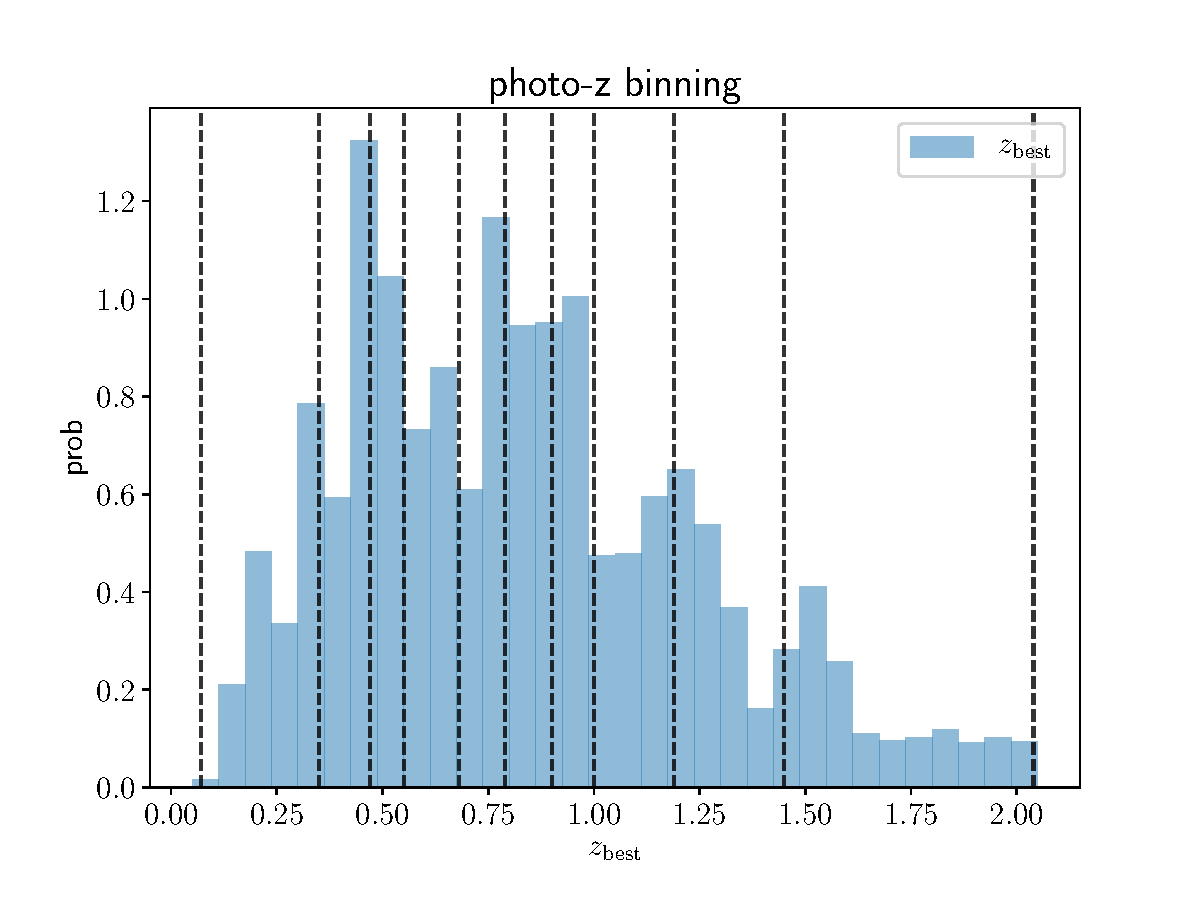
\includegraphics[height=.8\textwidth]{../paper_ms_method_HSCY1/photo-z_binning.pdf}
\end{column}
\begin{column}{0.5\textwidth}
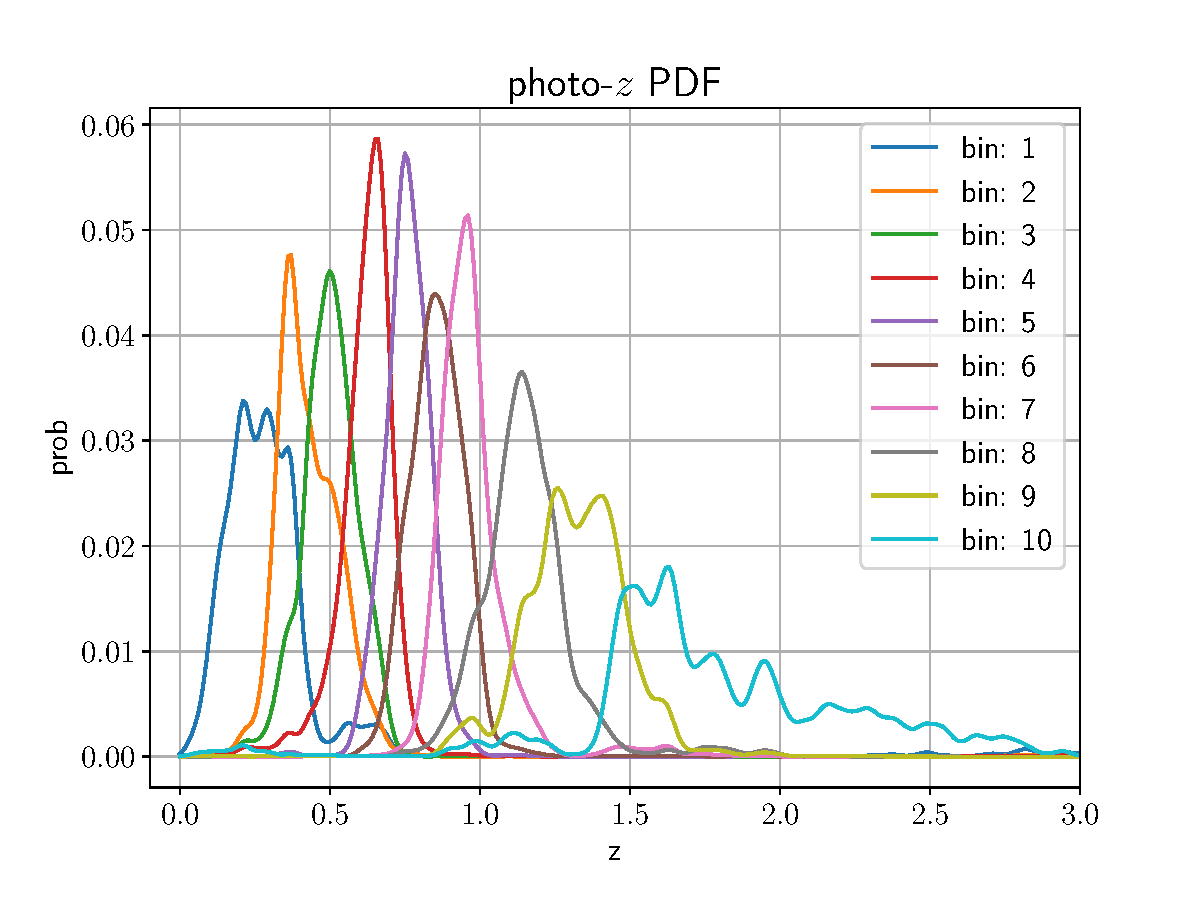
\includegraphics[height=.8\textwidth]{../paper_ms_method_HSCY1/mlz-poz.pdf}
\end{column}
\end{columns}
\end{frame}

\begin{frame}{Simulation}
\begin{columns}
\begin{column}{0.4\textwidth}
\begin{alertblock}{Photo-$z$ error}
$$n_{zp}(z)=\left\langle P(z|z_p) \right\rangle$$
\end{alertblock}
\end{column}
\begin{column}{0.6\textwidth}
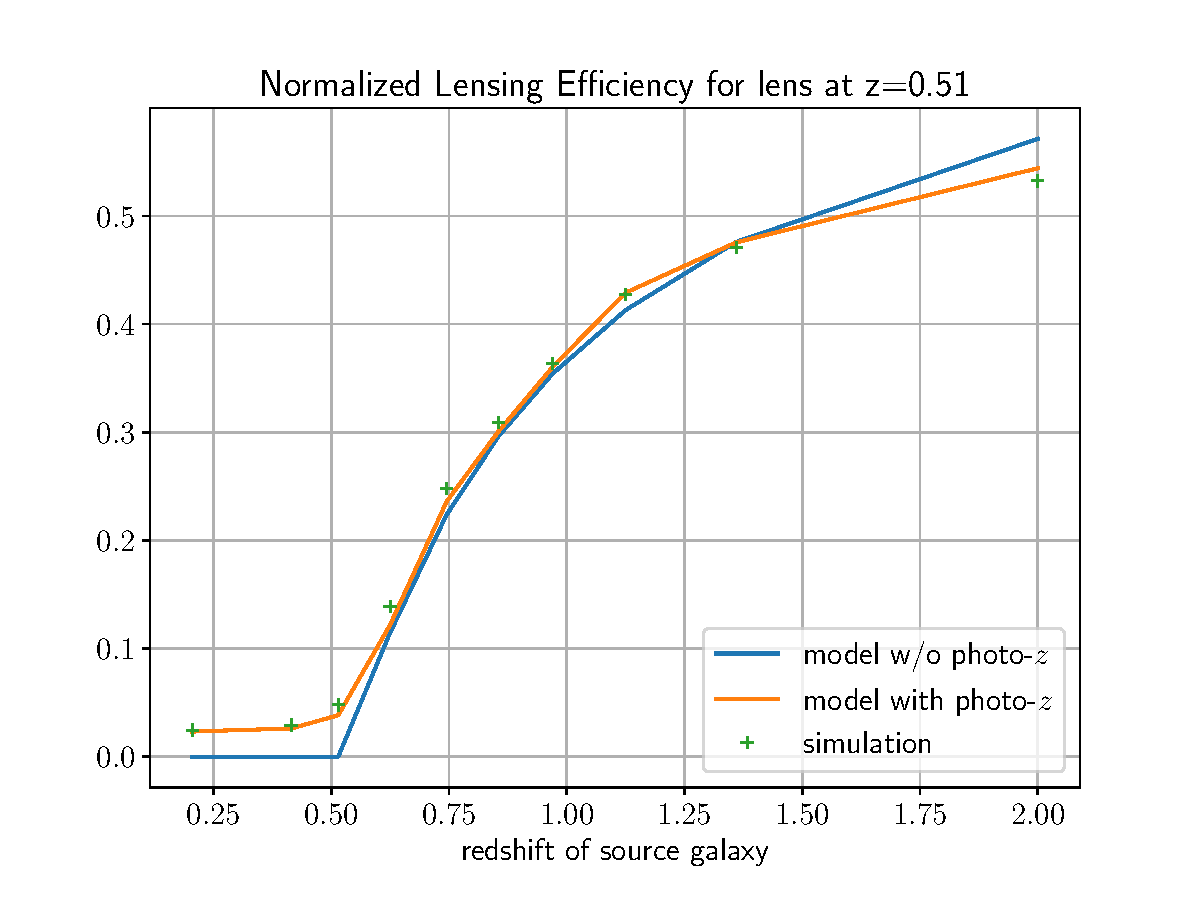
\includegraphics[height=.8\textwidth]{../paper_ms_method_HSCY1/lensing_efficiency.pdf}
\end{column}
\end{columns}
\end{frame}

\begin{frame}{Simulation}
\begin{columns}
\begin{column}{0.4\textwidth}

\begin{alertblock}{Noise}

\end{alertblock}

\end{column}
\begin{column}{0.6\textwidth}
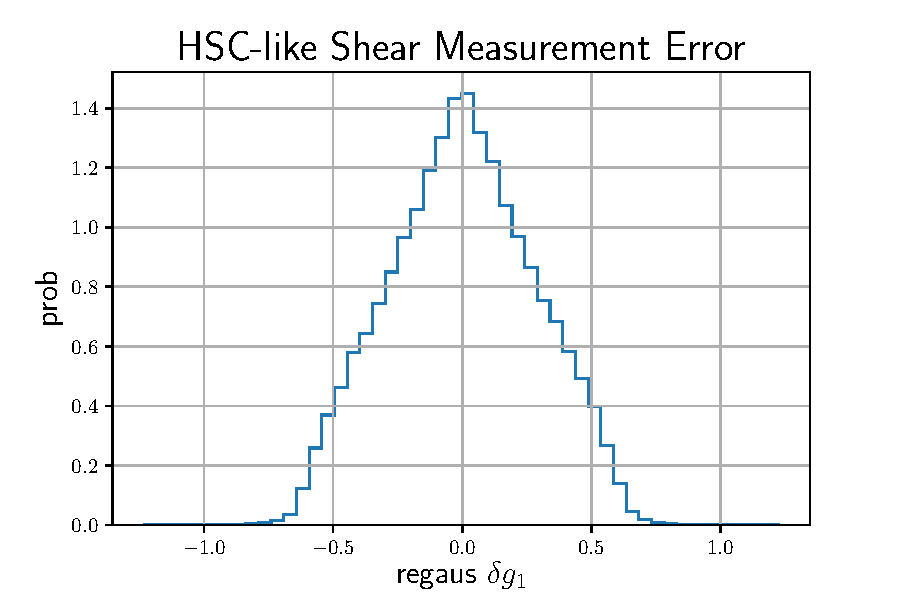
\includegraphics[height=.8\textwidth]{../paper_ms_method_HSCY1/shapeMeasurementError-HSCY1.pdf}
\end{column}
\end{columns}
\end{frame}

\begin{frame}{Outcomes1}
\begin{columns}
\begin{column}{0.5\textwidth}
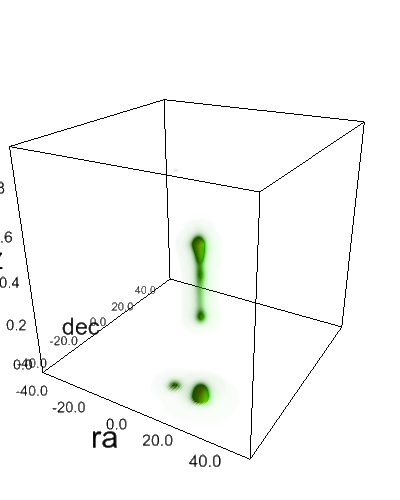
\includegraphics[height=1.\textwidth]{tau008-z3-m5.png}
\end{column}
\begin{column}{0.5\textwidth}
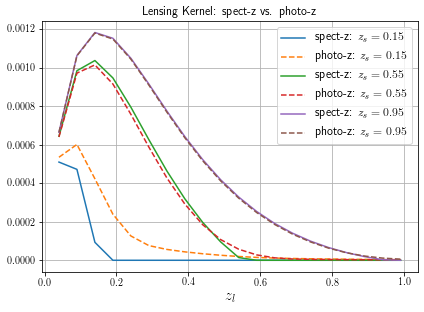
\includegraphics[height=.8\textwidth]{download.png}
\end{column}
\end{columns}
\end{frame}

\begin{frame}{Glimpse3D (Leonard et. al 2013)}

\begin{columns}
\begin{column}{0.5\textwidth}
\begin{itemize}
\item Begin with $x^{(0)}=0$, $s^{(0)}=0$
 \item for n=1...$N_{iter}$
    \begin{enumerate}
     \item choose the coordinate $t^{(n)}$ s.t. max\{$\frac{\partial_t G(x^{(n)})}{A_{\alpha t}A_{\alpha t}+4\tau}/(\sigma_t)$\}
     \item \begin{itemize}
            \item if $\rm{SNR_{max}}>s^{(n-1)}$: $s^{(n)}=(\rm{SNR_{max}}+\rm{SNR_{max2})/2}$
            \item ...
           \end{itemize}

    \end{enumerate}
\end{itemize}
\end{column}
\begin{column}{0.5\textwidth}
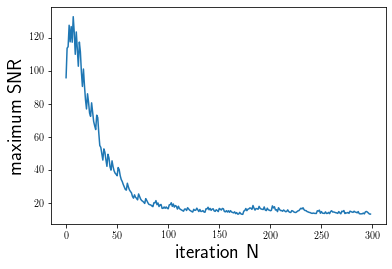
\includegraphics[height=.75\textwidth]{./tau20spect-maxSNR-z2-m8.png}
\end{column}
\end{columns}
\end{frame}

\begin{frame}{Outcomes2}
\begin{columns}
\begin{column}{0.32\textwidth}
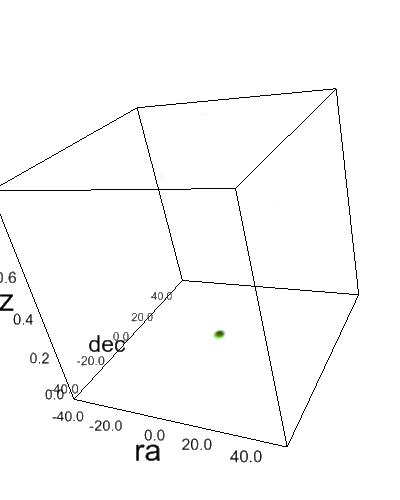
\includegraphics[height=.9\textwidth]{./tau20spect-z1-m4.png}
$z=0.01, logM=14.5$
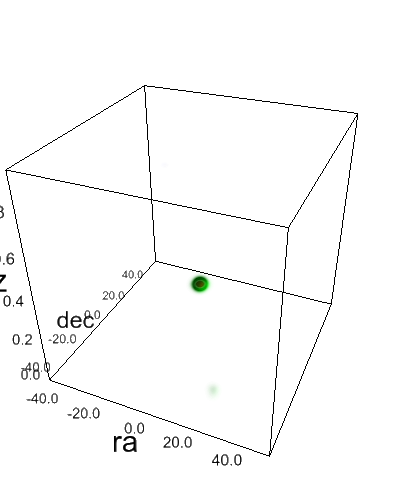
\includegraphics[height=.9\textwidth]{./tau20spect-z3-m5.png}
$z=0.26, logM=14.7$
\end{column}
\begin{column}{0.32\textwidth}
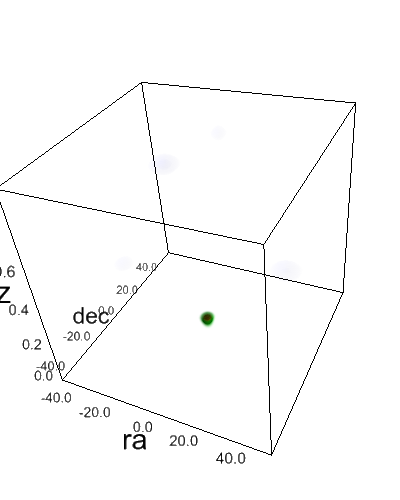
\includegraphics[height=.9\textwidth]{./tau20spect-z1-m7.png}
$z=0.01, logM=15.2$
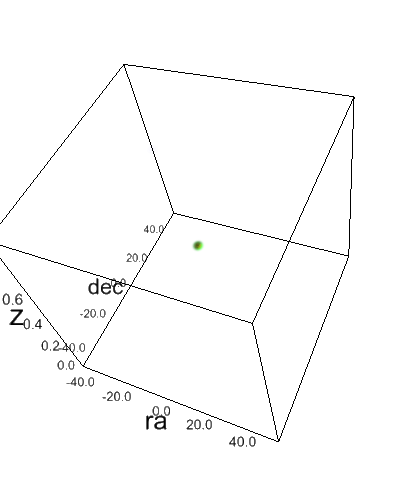
\includegraphics[height=.9\textwidth]{./tau20spect-z4-m7.png}
$z=0.51, logM=15.2$
\end{column}
\begin{column}{0.32\textwidth}
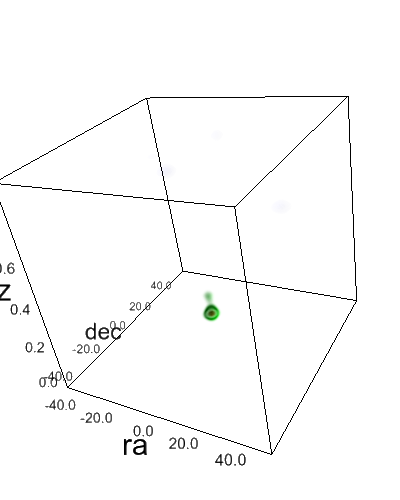
\includegraphics[height=.9\textwidth]{./tau20spect-z2-m8.png}
$z=0.13, logM=15.5$
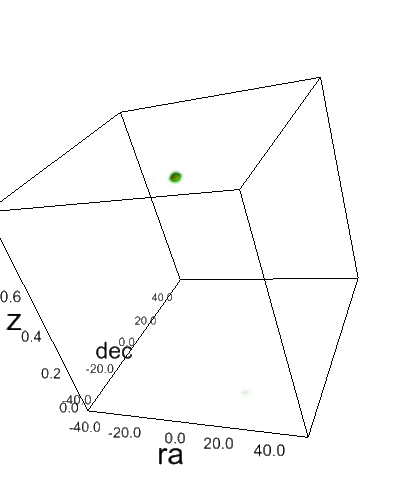
\includegraphics[height=.9\textwidth]{./tau20spect-z7-m7.png}
$z=0.88, logM=15.2$
\end{column}
\end{columns}
\end{frame}


\begin{frame}{}
Thanks!
\end{frame}



\end{document}
